\section{Results}
\label{sec-results}
In this section, we present the results obtained from carrying out our
methodology, and discuss some of the implications of our results.
Most of our results investigate the effect of an independent variable
(time-of-day and developer experience/frequency classifications) on
the likelihood of a commit to be a bug-introducing commit, or
\emph{bugginess}. We also
describe our findings with respect to the day of the week, which
allows us to compare our results to those
in~\cite{sliwerski-msr-2005}.  Finally, we explain the precision and
recall of our methodology and how we computed these figures.

\paragraph{Project characteristics}
We chose two large open-source software repositories for our
investigations: Linus Torvalds's mainline Linux kernel, from
\url{git.kernel.org} and PostgreSQL, from the project's repository at
\url{git.postgresql.org}. 


Table~\ref{tab:characteristics} summarizes
the characteristics of each of our repositories. 
Row ``bug-introducing'' shows that 23.7-25.5\% of the commits are buggy, which 
is slightly lower than the previously reported nearly 40\% for a commercial switching system~\cite{smallCommits05}. 
%of the samll commits are buggy, this number is on all commits
%in the previous work by Purushothaman and Perry~\cite{smallCommits05}.
Note that the
PostgreSQL repository was carefully converted from CVS using {\code cvs2git} in
September 2010. We discussed some of the quirks of the PostgreSQL repository
in Section~\ref{sec:method}.


\begin{table}
\begin{tabular}{l|r|r}
& {\bf Linux} & {\bf PostgreSQL} \\ \hline
First commit & April 16, 2005 & July 9, 1996 \\
Cloned & November 21, 2010 & January 24, 2011 \\
Lines of code at tip & over 5 million & over 750,000 \\
%Source & \url{git.kernel.org} & \url{git.postgresql.org} \\
Number of authors & 8,594 & 34 \\
Number of commits & 222,332 & 31,098 \\
\# bug-introducing & 56,681 (25.5\%) & 7,366 (23.7\%) \\
\# bug-fixing & \linuxBFC & \postBFC
\end{tabular}
\caption{\label{tab:characteristics}Characteristics of the Linux kernel and PostgreSQL repositories.}
\end{table}

%% The Linux repository
%% was cloned on November 21, 2010, from Linus Torvalds's mainline
%% kernel, hosted at \url{git.kernel.org}; this repository contains
%% history back to April 16, 2005.  This repository contains 222,332
%% commits contributed by 8,594 authors. Of these commits, we identified
%% 56,681 bug-introducing commits and 57,028 bug-fixing commits.
%% The tip of the repository contains
%% over 5 million lines of code. 

%% The PostgreSQL repository was cloned on January 24, 2011, from the
%% project's repository at \url{git.postgresql.org}; it contains history
%% to July 9, 1996, translated from CVS using \code{cvs2git}.  This
%% repository contains 31,098 commits contributed by 34 authors. We
%% identified 7,366 bug-introducing commits and 4,399 bug-fixing commits. The tip
%% of the repository contains over 750,000 lines of code.

\subsection{Time-of-day Results} 
\label{sec-time-of-day}
We first present our results correlating the time-of-day of a commit
with its bugginess.  
Figures~\ref{fig-linux-bugginess-hour}
and~\ref{fig-postgresql-bugginess-hour} present results from the Linux kernel and
Postgres, respectively. These graphs compare the time-of-day of each
commit, in the committer's local time on a 24-hour clock, to the
percentage of commits which were found to be bug-introducing. The
solid horizontal line indicates the overall percentage number of buggy commits in
each project; bars shorter than the line indicate that commits at that
hour were less likely to be buggy, while bars taller than the line
indicate hours with more-buggy commits. The graphs also contain the
raw number of commits at each hour, as indicated by the red dots.

While our principal metrics are the absolute count and percentage of
bug-introducing commits, we also present results of a third metric,
\emph{bug severity}. This metric attributes less weight to a large
commit which introduces a small number of bugs relative to its size,
and more weight to small commits which introduce relatively large
numbers of bugs. We define bug severity to be the number of bug
introductions per changed non-comment lines of
code. Figure~\ref{fig-severity-hour} presents our data correlating
severity of changes, along with average commit size, with time-of-day.

Figures~\ref{fig-linux-bugginess-hour}
and~\ref{fig-postgresql-bugginess-hour}, summarizing bugginess
percentages, show a noticeable increase in the amount of commits which
introduce a bug between 00:00 (midnight) and 04:00 (4AM). After 04:00,
commits tend to be less buggy than average, gradually increasing until
noon.  In the Linux kernel, commits between noon and midnight
fluctuate around the average bugginess level, while the Postgres
commits are generally above the average bugginess level between 16:00
(4PM) and 20:00 (8PM), and then below the average bugginess level
between 20:00 (8PM) and 00:00
(midnight). Figures~\ref{fig-linux-introduction-hour}
and~\ref{fig-postgresql-introduction-hour} track the trends in
Figures~\ref{fig-linux-bugginess-hour}
and~\ref{fig-postgresql-bugginess-hour}. Note that even the smallest
total number of commits, for any hour, is 139 for Postgres (and an
order of magnitude higher for the Linux kernel), so that all of the
depicted bug introduction rates are meaningful.

Figures~\ref{fig-linux-severity-hour}
and~\ref{fig-postgresql-severity-hour} show that the severity of
late-night/early-morning changes (before 9AM) is surprisingly high,
while there is no general trend in the average commit size.
The average size of Linux commits fluctuates quite a lot; the sizes of
Postgres commits are more stable.  For Postgres, developers tend to
commit slightly smaller changes between 5AM and noon, with a spike at 8AM.

These results indicate that developers may want to double check the code they write for these 
late-night commits (0:00-4:00 AM).
It may also be beneficial for the version control
system to warn the developers of late-night commits to improve software reliability. 

Our results may suggest that tired developers (midnight-4AM) are more
likely to miss corner cases in a pre-commit review (for Postgres) or
while finalizing the patch (for the Linux kernel). Furthermore, we can observe
that commits before noon are least likely to be bug-introducing;
perhaps committers are most careful in those hours.
%While we believe the above observations are true, we do not draw  
%

We also investigated correlations between the time-of-day and the
number of bug-fixing commits, rather than the bug-introducing commits
that we showed above. We found that the proportion of total
commits that are bug-fixing commits stayed almost constant independent
of the hour; the graphs (not shown) have exactly the same shape as
that of the circles in Figures~\ref{fig-bugginess-hour}.
%and~\ref{fig-postgresql-bugginess-hour}. 
This suggests that the fact
that a commit is bug-fixing does not affect its other characteristics.

\begin{figure*}[tbh]
\centering
\subfigure [ {Linux kernel} ]  
{
    \label{fig-linux-bugginess-hour}
     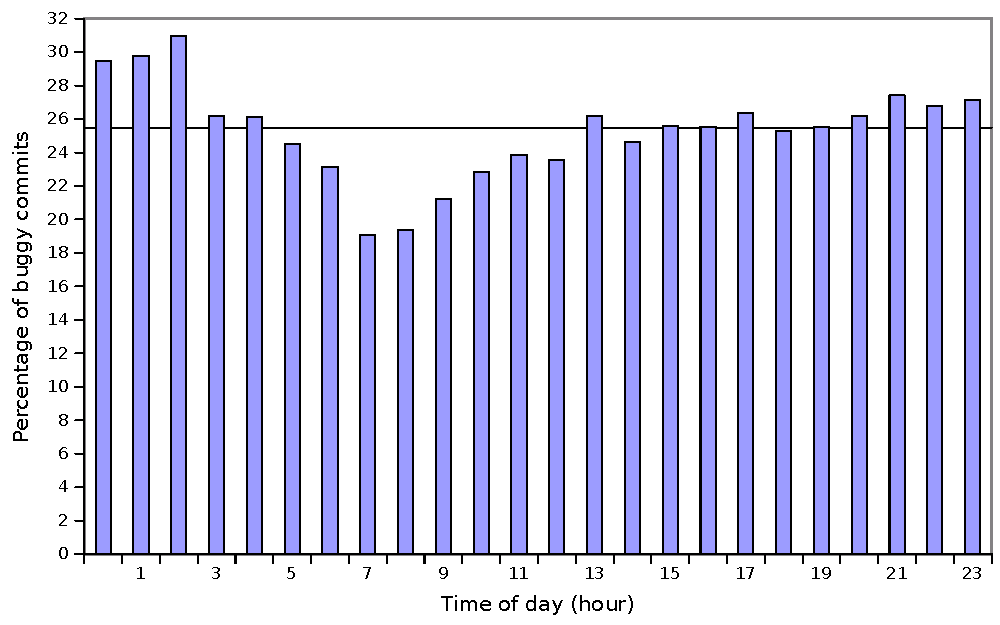
\includegraphics[width=\columnwidth]{linux-bugginess-hour.pdf}
}
\subfigure[ PostgreSQL ] 
{
    \label{fig-postgresql-bugginess-hour}
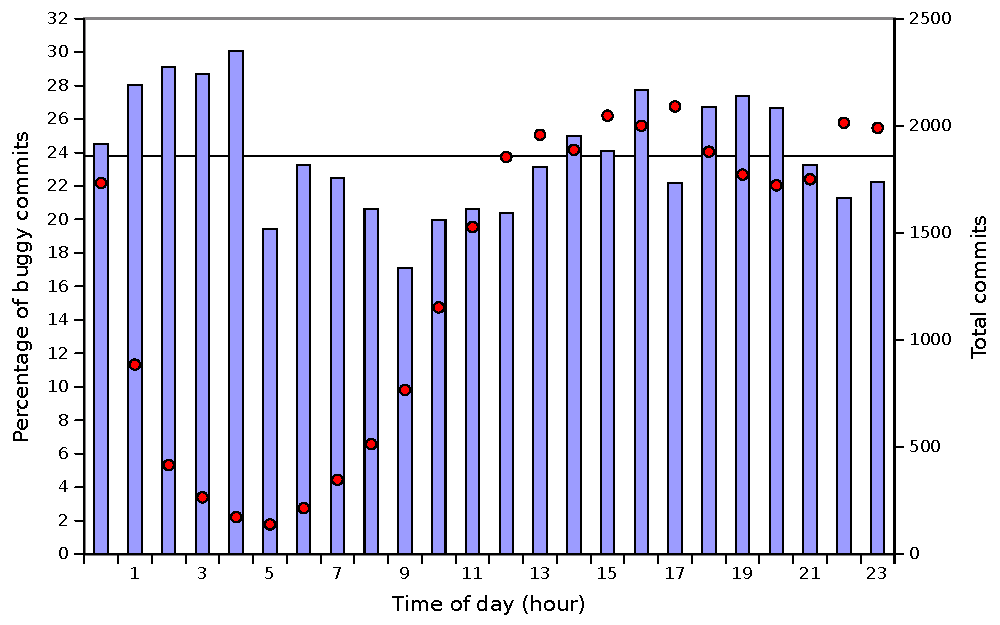
\includegraphics[width=\columnwidth]{postgresql-bugginess-hour.pdf}
}
\caption{The percentage of buggy commits (bars) and total number of commits (circles) versus time-of-day}
\label{fig-bugginess-hour} % caption for the whole figure
\end{figure*}

%----- introduction hour
\begin{figure*}[tbh]
\centering
\subfigure [ {Linux kernel} ]  
{
    \label{fig-linux-introduction-hour}
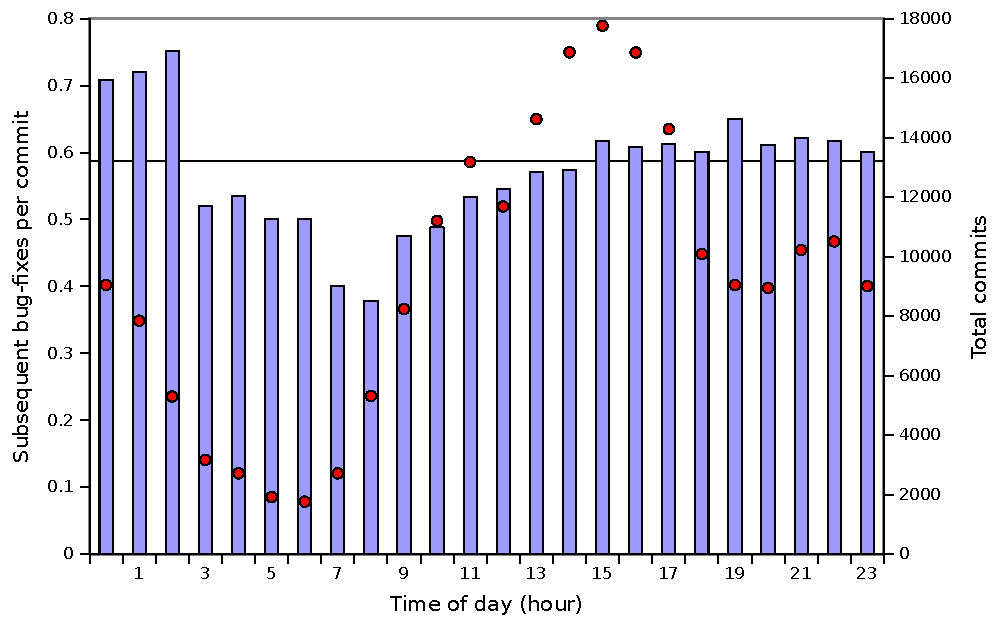
\includegraphics[width=\columnwidth]{linux-introductions-hour.pdf}
}
\subfigure[ PostgreSQL ] 
{
    \label{fig-postgresql-introduction-hour}
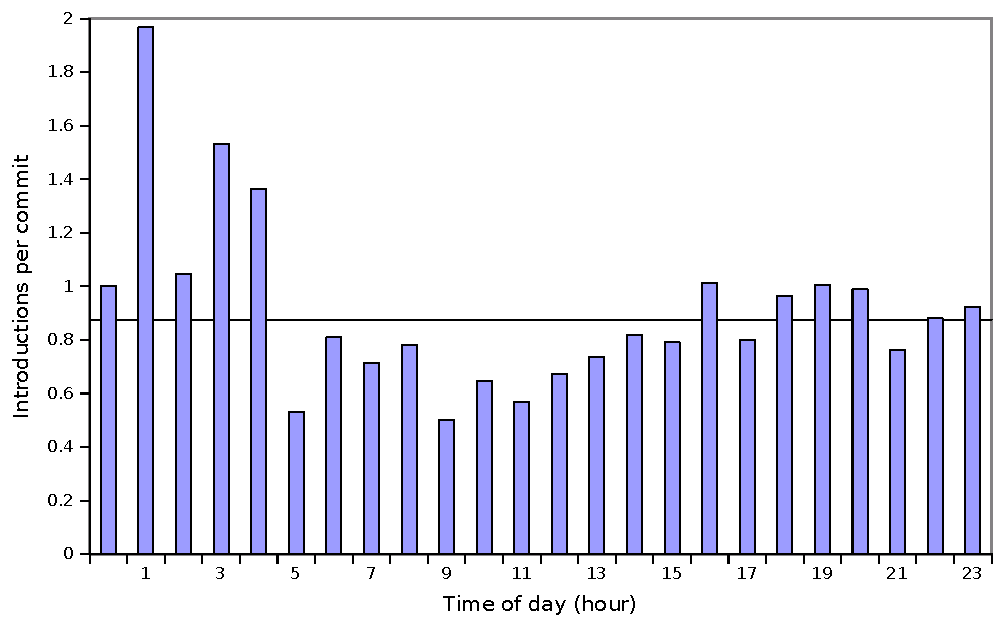
\includegraphics[width=\columnwidth]{postgresql-introductions-hour.pdf}
}
\caption{Bug introductions per commit (bars) and total commits (circles) versus time-of-day}
\label{fig-introduction-hour} % caption for the whole figure
\end{figure*}

%------ severity hour 
\begin{figure*}[tbh]
\centering
\subfigure [ {Linux kernel} ]  
{
    \label{fig-linux-severity-hour}
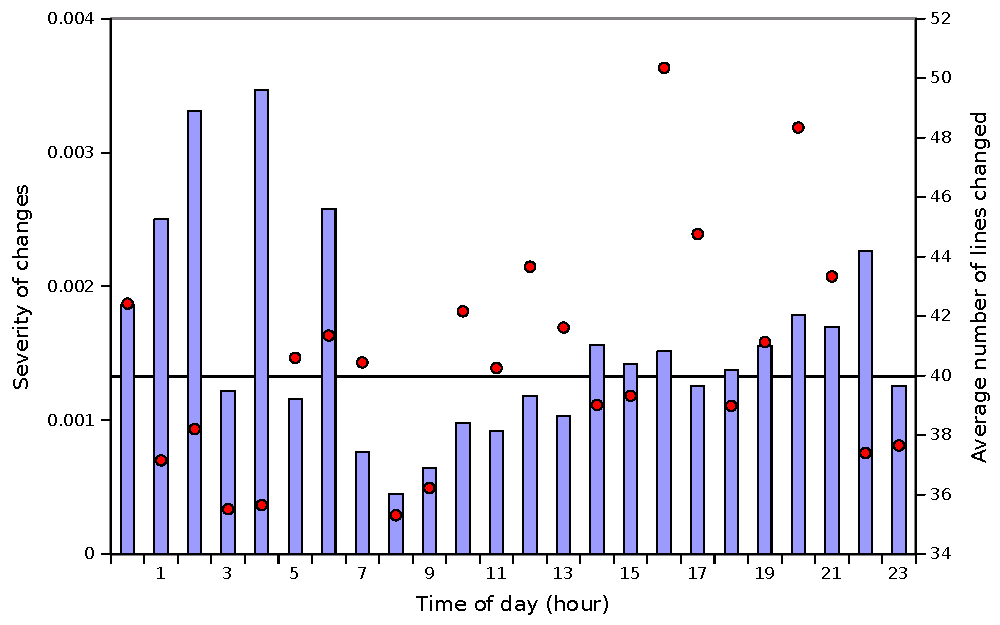
\includegraphics[width=\columnwidth]{linux-severity-hour.pdf}
}
\subfigure[ PostgreSQL ] 
{
    \label{fig-postgresql-severity-hour}
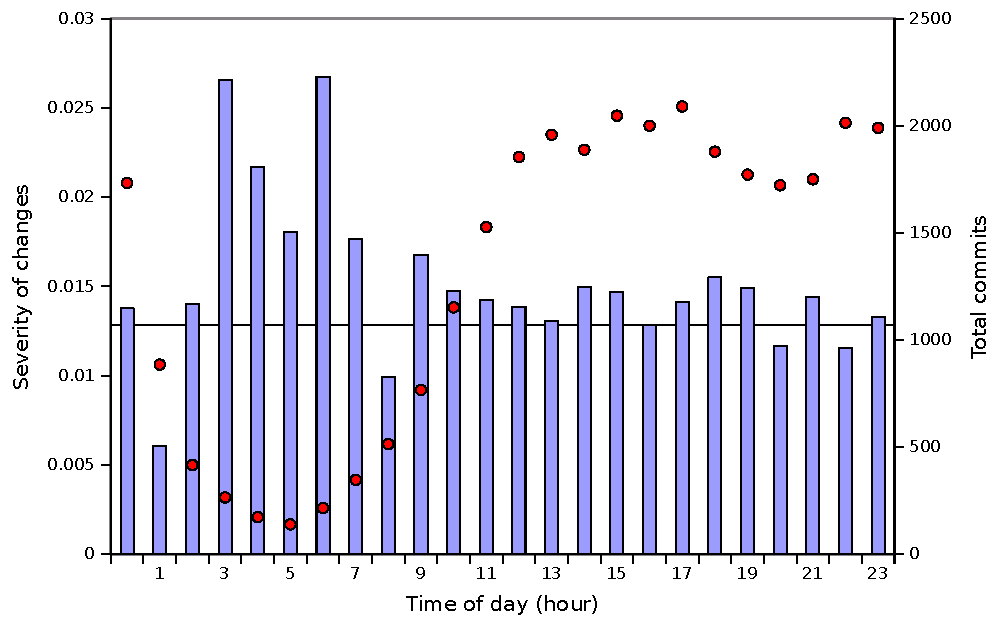
\includegraphics[width=\columnwidth]{postgresql-severity-hour.pdf}
}
\caption{Severity of changes (bars) and average number of lines per commit (circles) versus time-of-day}
\label{fig-severity-hour} % caption for the whole figure
\end{figure*}

%% \begin{figure}
%% \begin{center}
%% 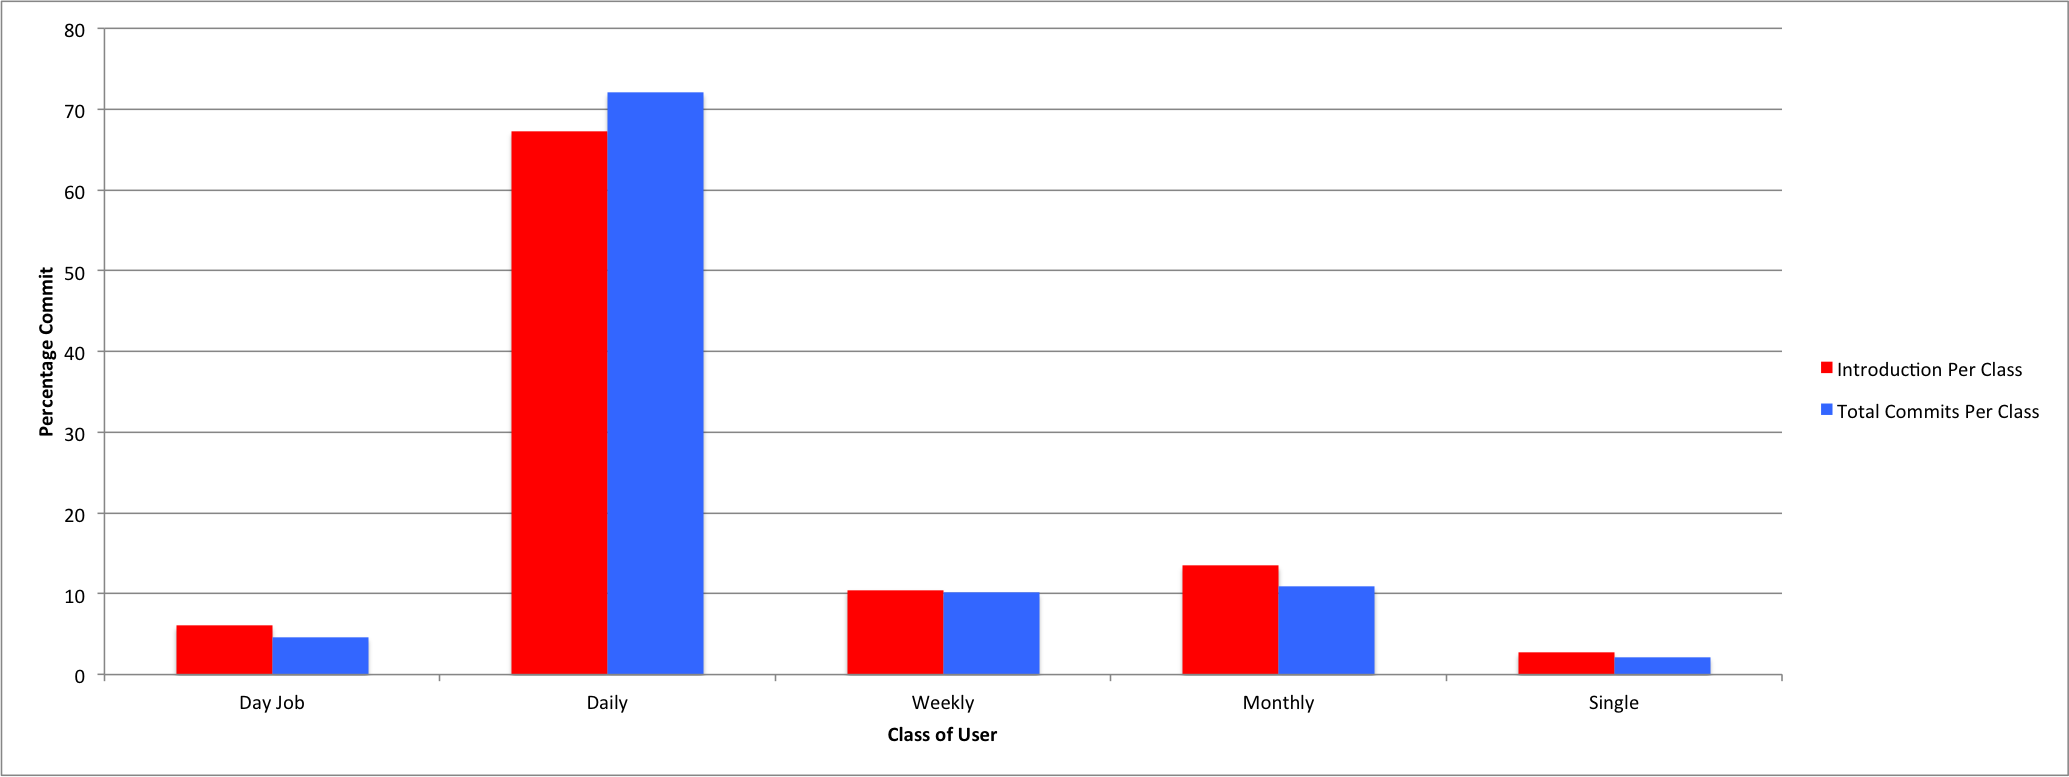
\includegraphics[width=0.45\textwidth]{linux_per_class.png}
%% \end{center}
%% \caption{Linux percentage of bug introductions and percentage of total commits per author classification}
%% \label{fig-linux-class}
%% \end{figure}

%% \begin{figure}
%% \begin{center}
%% 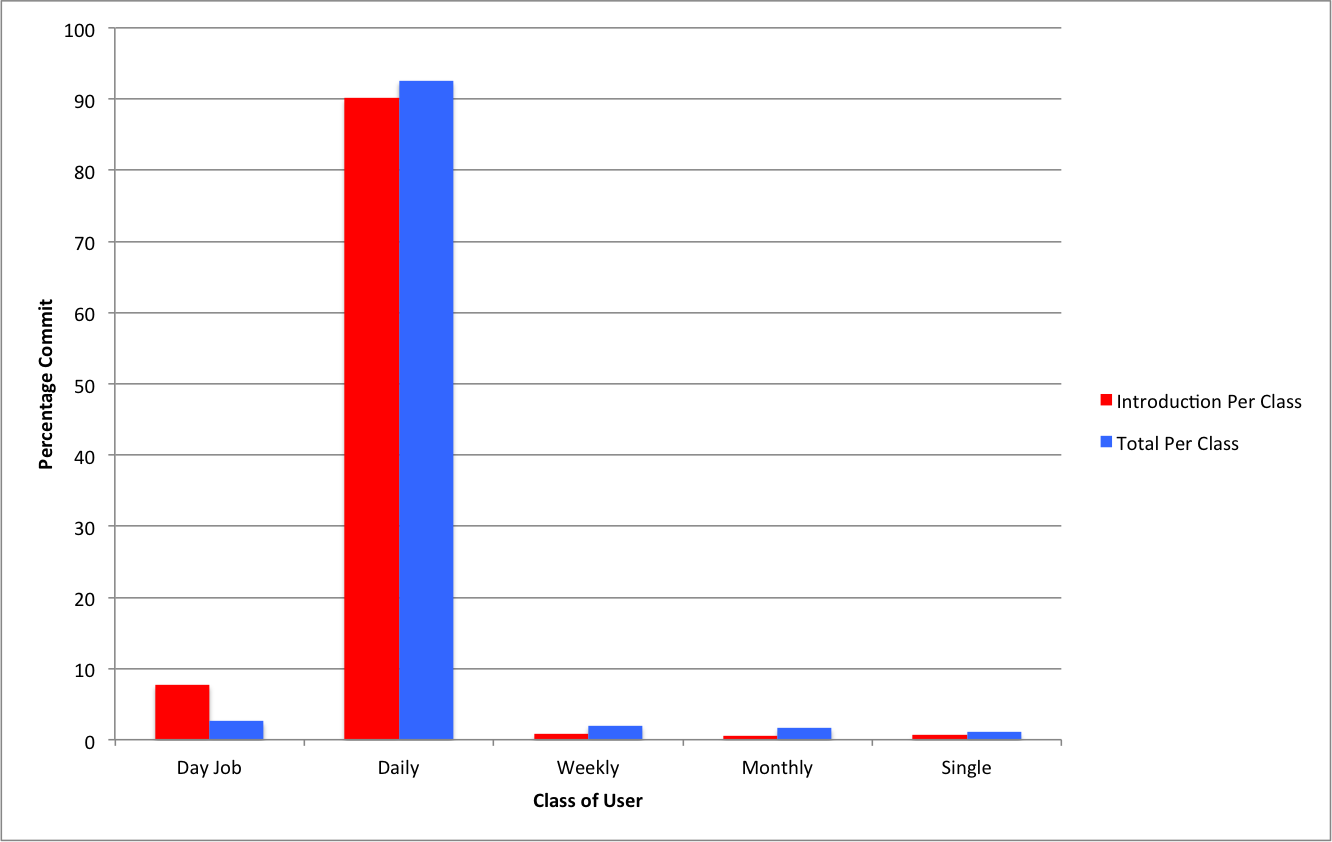
\includegraphics[width=0.45\textwidth]{firefox_per_class.png}
%% \end{center}
%% \caption{Firefox percentage of bug introductions and percentage of total commits per author classification}
%% \label{fig-firefox-class}
%% \end{figure}

\subsection{Developer Characteristics}
\label{sec-dev-char}
We next present our findings with respect to developers' commiting 
frequency and experience classification. Developers'
commiting frequency summarizes the frequency of
a developer's contributions to a project, while developer experience
tracks how long a developer has contributed to a particular project.

\paragraph{Commit Frequency Classification} 
As we described in Section~\ref{sec:data}, one of the ways that we
classify developers is according to frequency, i.e. most-common
interval between consecutive commits---daily, weekly, monthly, other,
or single.  This information is only interesting for the Linux kernel,
as almost all (28/34) of Postgres's committers are daily. We computed
the bugginess rates for each of these classes of developers and plot
author classification versus bug-introduction percentage in
Figure~\ref{fig-linux-bugginess-author-class}. The graph also presents
the number of commits by each class. Note that the Linux kernel has 49
day job authors, who provide quite a few of the total commits, and 238
weekly and 288 monthly authors.

Our results show that the Linux kernel developers who commit changes daily, but
not as their day job, produce the smallest number of bug-introducing
commits, followed by the single-commit authors (whose patches would
presumably be simple or closely-reviewed). The day job, weekly, and
monthly committers all produce slightly more bug-introducing commits
than average.

A possible cause for the difference between day-job and daily
committers is that day-job developers might be required to make
changes by their employers, while the daily developers are motivated
purely by interest, and unlikely to be pressured to fix bugs on any
particular schedule.

\begin{figure}
\begin{center}
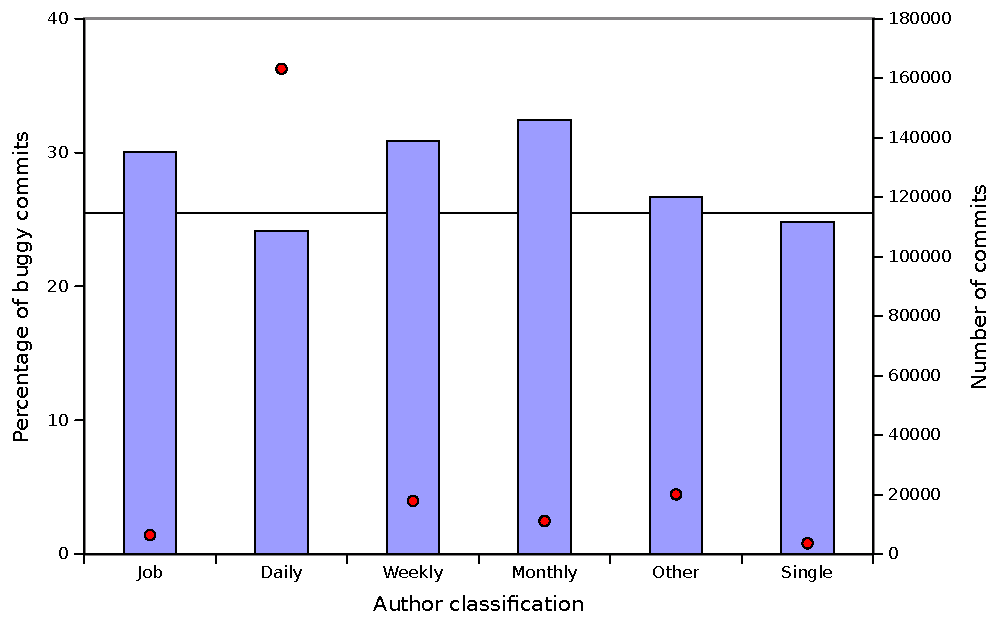
\includegraphics[width=\columnwidth]{linux-bugginess-author-class.pdf}
\end{center}
\caption{Linux percentage of buggy commits (bars) and number of authors (circles) versus author classification}
\label{fig-linux-bugginess-author-class}
\end{figure}

% we need to say what the two bars mean in the figure.

%% \begin{figure}
%% \begin{center}
%% 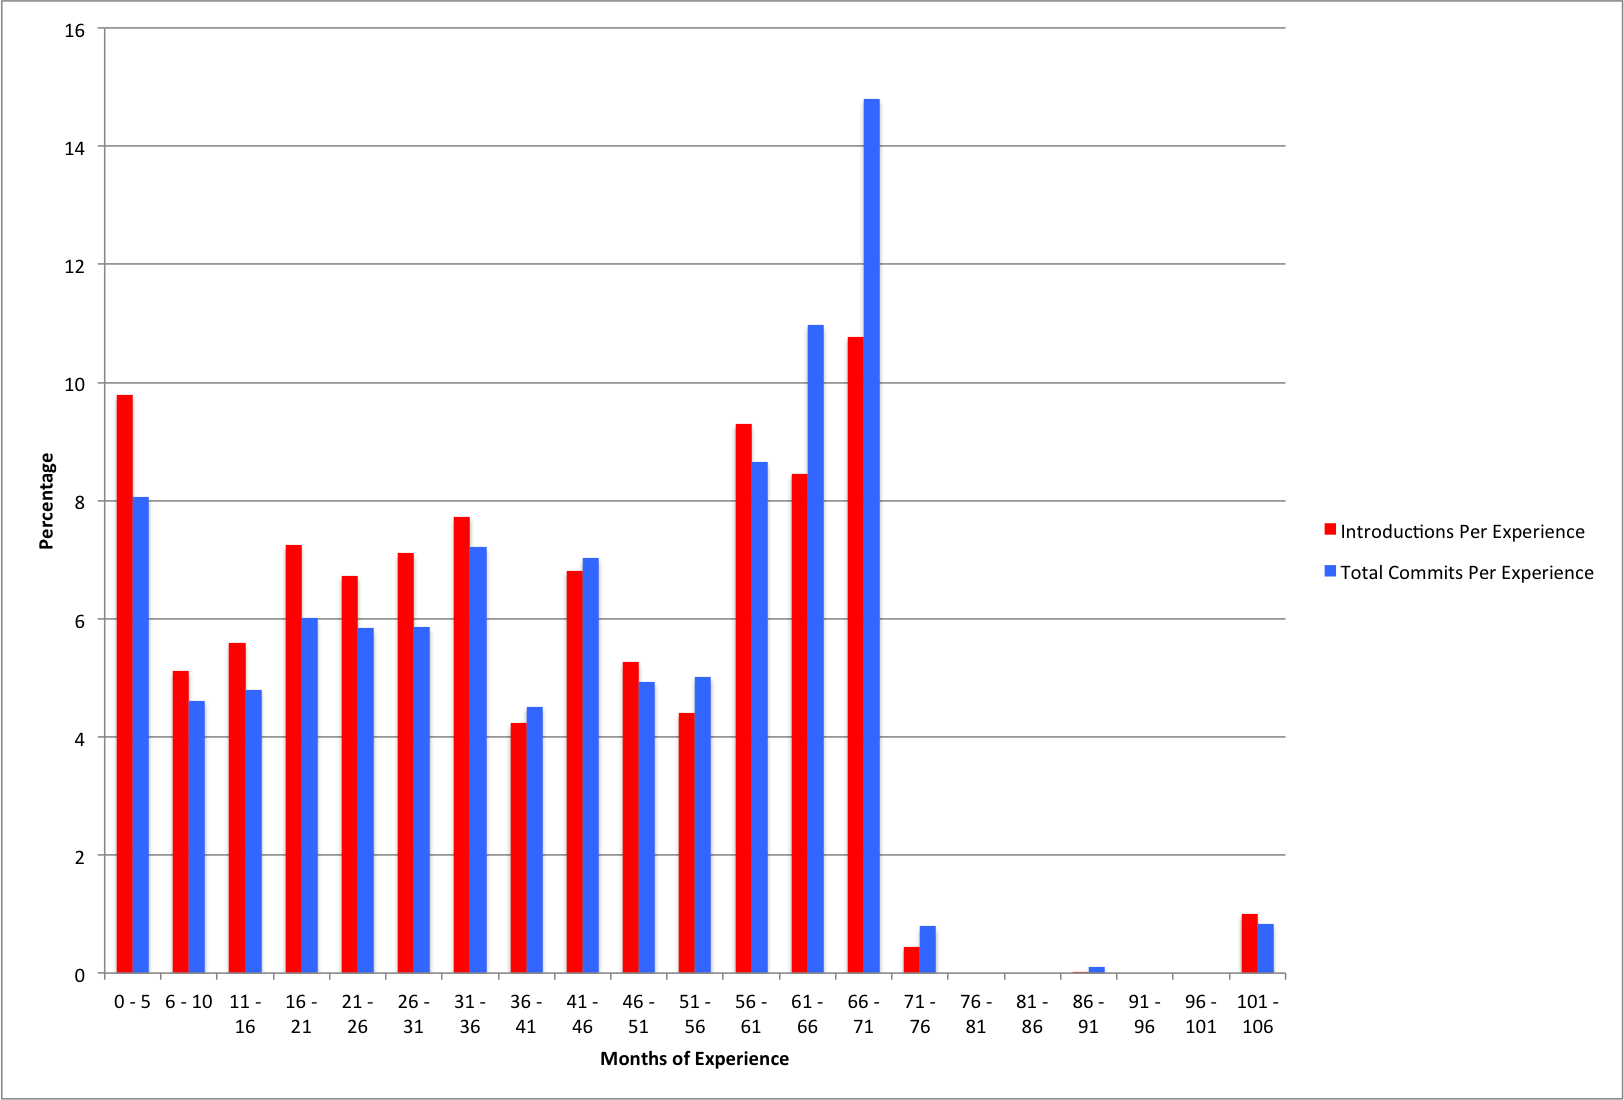
\includegraphics[width=0.45\textwidth]{linux_day_per_experience.png}
%% \end{center}
%% \caption{Linux percentage of bug introductions and percentage of total commits per author experience}
%% \label{fig-linux-experience}
%% \end{figure}

%% \begin{figure}
%% \begin{center}
%% 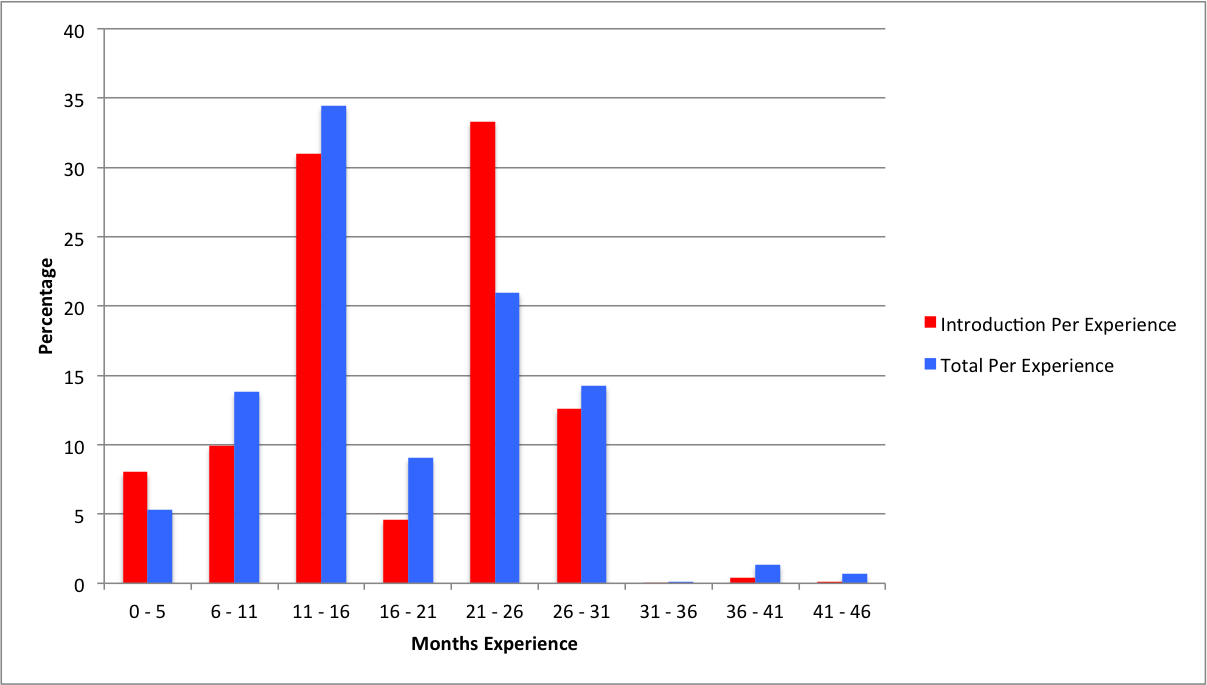
\includegraphics[width=0.45\textwidth]{firefox_day_per_experience.png}
%% \end{center}
%% \caption{Firefox percentage of bug introductions and percentage of total commits per author experience}
%% \label{fig-firefox-experience}
%% \end{figure}

\paragraph{Developer Experience Classification}

Figure~\ref{fig-bugginess-experience} %and Figure~\ref{fig-postgresql-bugginess-experience} 
shows that, in general, the more experienced the developers are, the less likely that their commits are buggy.
Without further data, this correlation does not prove that the developer experience caused more 
experienced programmers' commits to be less buggy. 
While we believe the above causation to hold, other interpretations are possible; perhaps more experienced developers wrote 
more complex code, whose bugs are harder to discover and less likely to be reported. 
Nonetheless, our results show that given the fact that a commit is from a more experience developer, 
one can be more confident about the correctness of the commit. Such a correlation could be exploited 
to help predict buggy code locations.


%% \begin{figure}
%% \begin{center}
%% 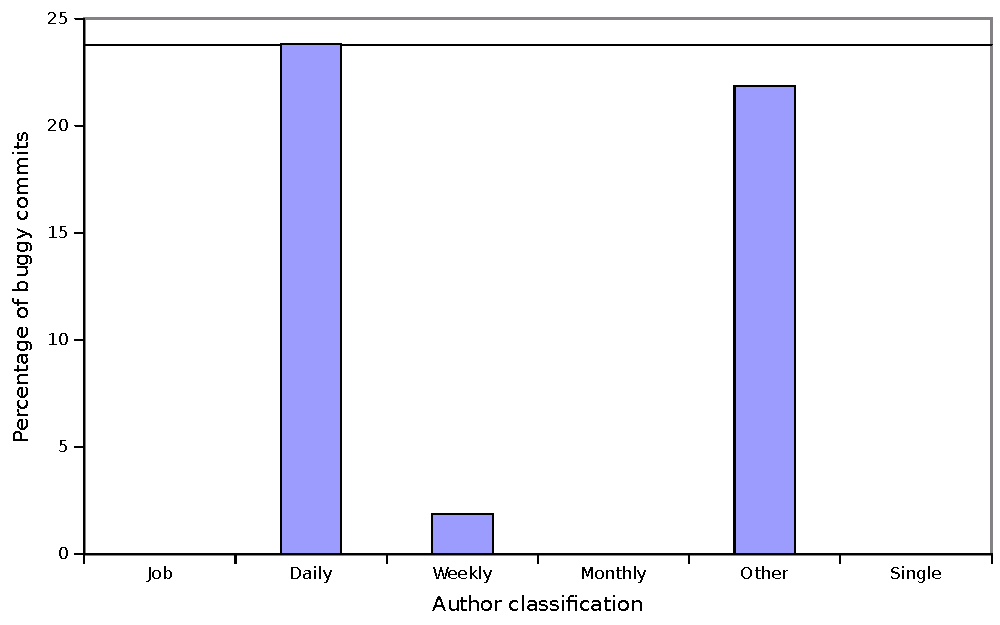
\includegraphics[width=0.45\textwidth]{postgresql-bugginess-author-class.pdf}
%% \end{center}
%% \caption{PostgreSQL percentage of buggy commits per author classification}
%% \label{fig-postgresql-bugginess-author-class}
%% \end{figure}


\begin{figure*}[tbh]
\centering
\subfigure [ {Linux kernel} ]  
{
    \label{fig-linux-bugginess-experience}
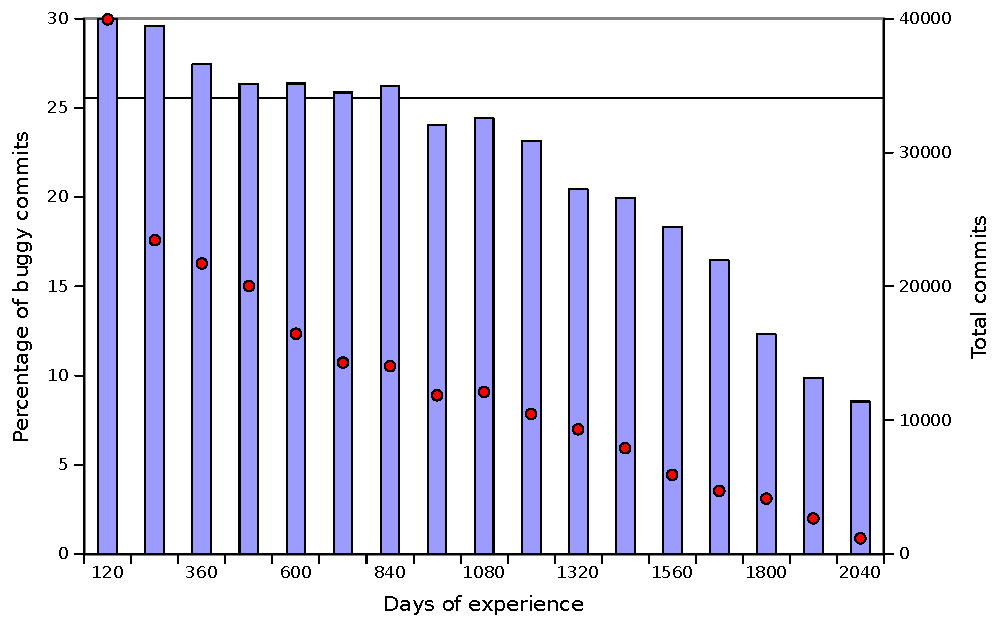
\includegraphics[width=\columnwidth]{linux-bugginess-experience.pdf}
}
\subfigure[ PostgreSQL ] 
{
    \label{fig-postgresql-bugginess-experience}
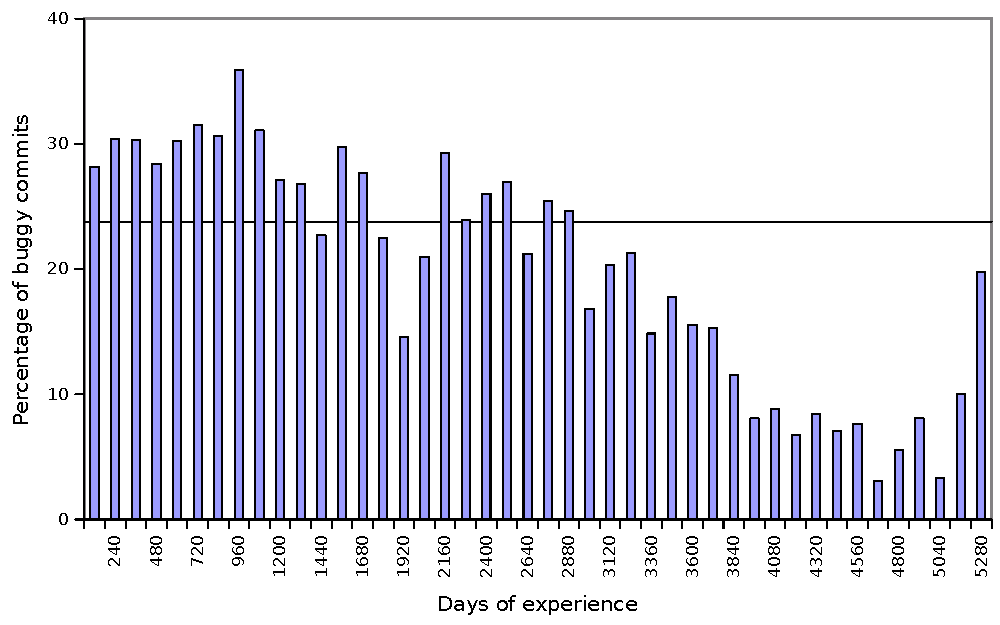
\includegraphics[width=\columnwidth]{postgresql-bugginess-experience.pdf}
}
\caption{Percentage of buggy commits (bars) and total number of commits (circles) versus author experience}
\label{fig-bugginess-experience} % caption for the whole figure
\end{figure*}





\subsection{Day-of-week Results}
\label{sec-day-of-week}
Our next experiment attempted to replicate the results
in~\cite{sliwerski-msr-2005} and correlates the day of the week
of a commit with its bugginess. Figures~\ref{fig-linux-bugginess-day} 
and~\ref{fig-postgresql-bugginess-day} compare the day of the week
with the bugginess of the commits on that day (bars) and also display
the total number of commits per day (dots). Once again, the solid
horizontal line presents the average bugginess of all commits to
each project.

Our results, which use a disjoint set of repositories from those
in~\cite{sliwerski-msr-2005}, found about the same bugginess for each
day in the Linux repository, with the lowest bugginess on Sunday and
highest on Monday and Thursday; for the Postgres repository, we
observe a slight decrease in bugginess on Saturday and Monday, a small
increase on Tuesday and Wednesday, and a noticeable increase on
Sunday.  Note that, for Linux, Saturday and Sunday each have about
half as many commits as the other days of the week (commits peak on
Tuesday and steadily decrease through Friday). For Postgres, commits
fluctuate through the days of the week and decrease to about 70\% of
the weekday volume on the weekend.

%{\bf Finding \fday and Implications:} 
In summary, commits on different days of week have the same level of bugginess, which
do not agree with results from the prior study on two different open source projects~\cite{sliwerski-msr-2005}.  
This result shows that the day of week of commits
vary for different software projects, implying that the bugginess prediction based on 
the day of week of commits may need to be on a project-by-project basis.


%---- bugginess day
\begin{figure*}[tbh]
\centering
\subfigure [ {Linux kernel} ]  
{
    \label{fig-linux-bugginess-day}
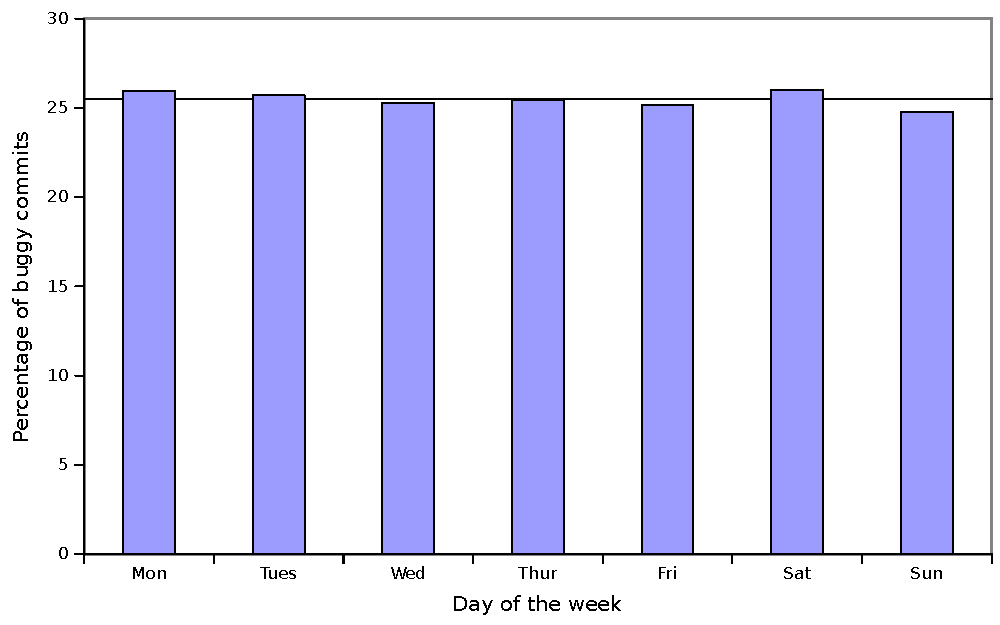
\includegraphics[width=\columnwidth]{linux-bugginess-day.pdf}
}
\subfigure[ PostgreSQL ] 
{
    \label{fig-postgresql-bugginess-day}
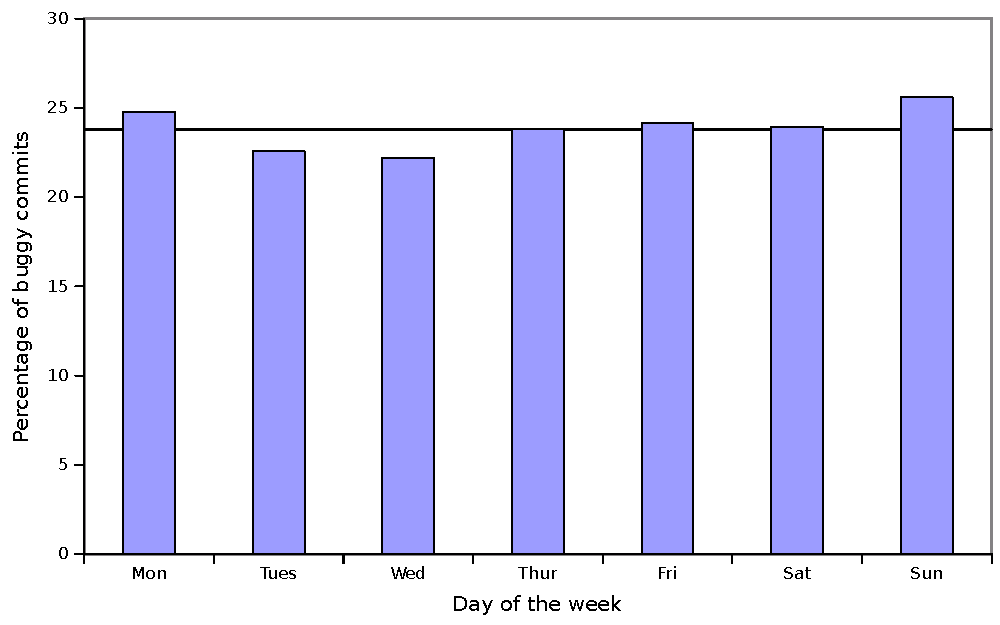
\includegraphics[width=\columnwidth]{postgresql-bugginess-day.pdf}
}
\caption{Percentage of buggy commits (bars) and total commits (circles) versus day-of-week}
\label{fig-bugginess-day} % caption for the whole figure
\end{figure*}

%--- introduction day
\begin{figure*}[tbh]
\centering
\subfigure [ {Linux kernel} ]  
{
    \label{fig-linux-introduction-day}
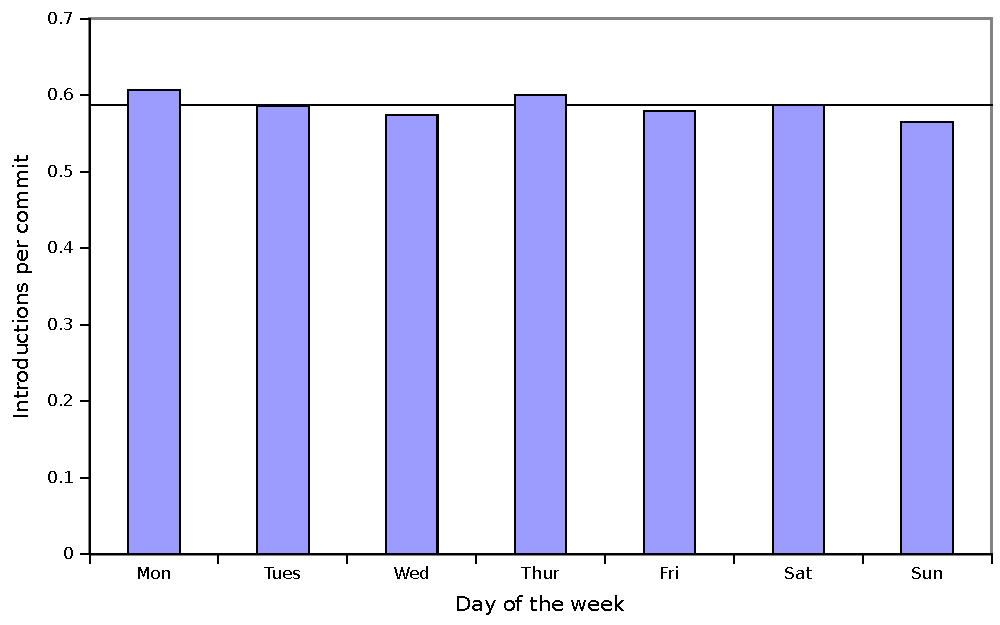
\includegraphics[width=\columnwidth]{linux-introductions-day.pdf}
}
\subfigure[ PostgreSQL ] 
{
    \label{fig-postgresql-introduction-day}
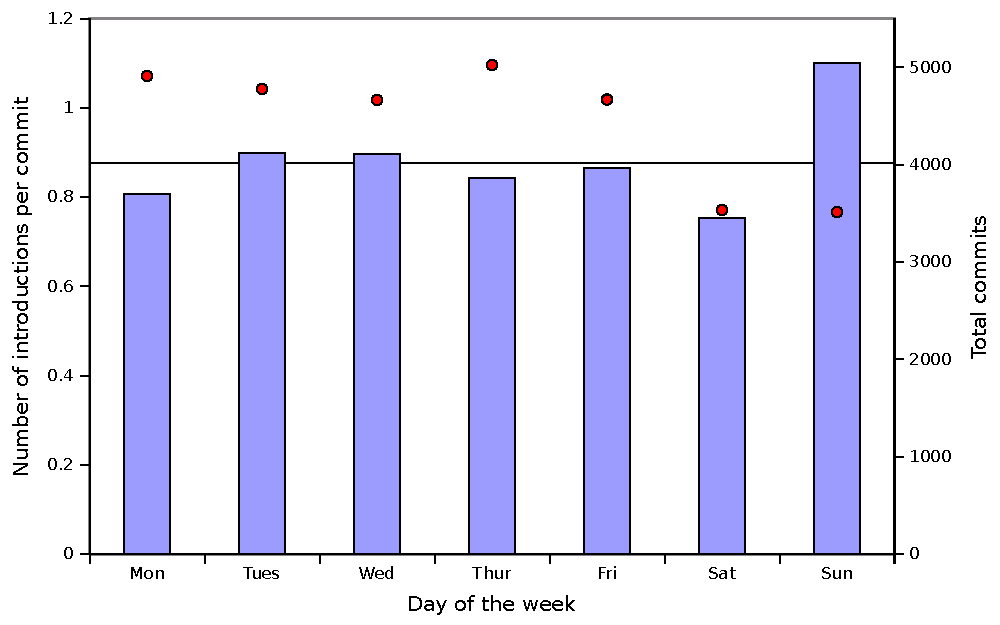
\includegraphics[width=\columnwidth]{postgresql-introductions-day.pdf}
}
\caption{Number of bug-introducing commits (bars) and total commits (circles) versus day-of-week}
\label{fig-introduction-day} % caption for the whole figure
\end{figure*}

%------ severity day
\begin{figure*}[tbh]
\centering
\subfigure [ {Linux kernel} ]  
{
    \label{fig-linux-severity-day}
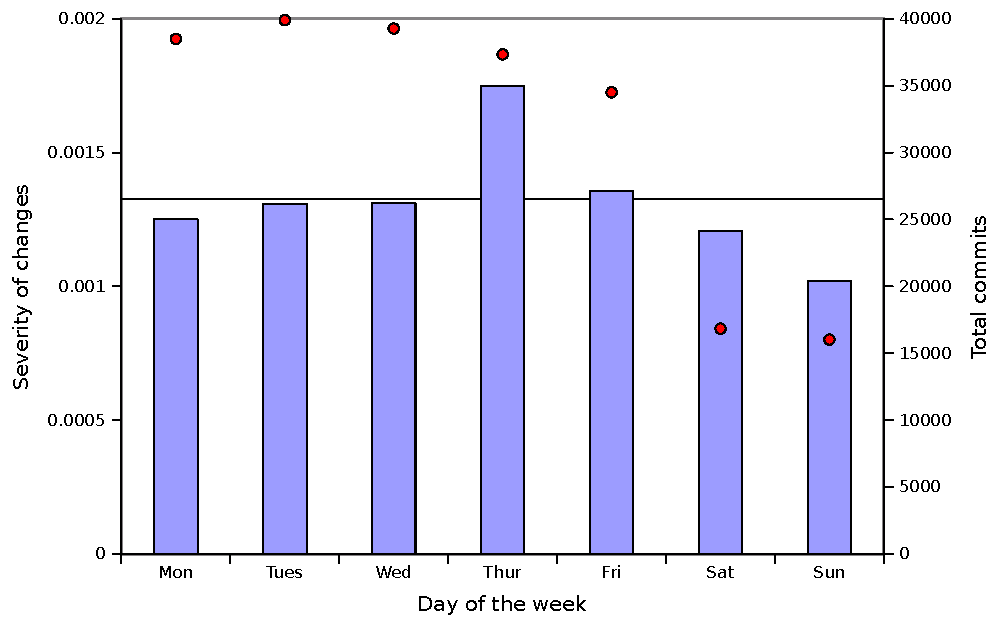
\includegraphics[width=\columnwidth]{linux-severity-day.pdf}
}
\subfigure[ PostgreSQL ] 
{
    \label{fig-postgresql-severity-day}
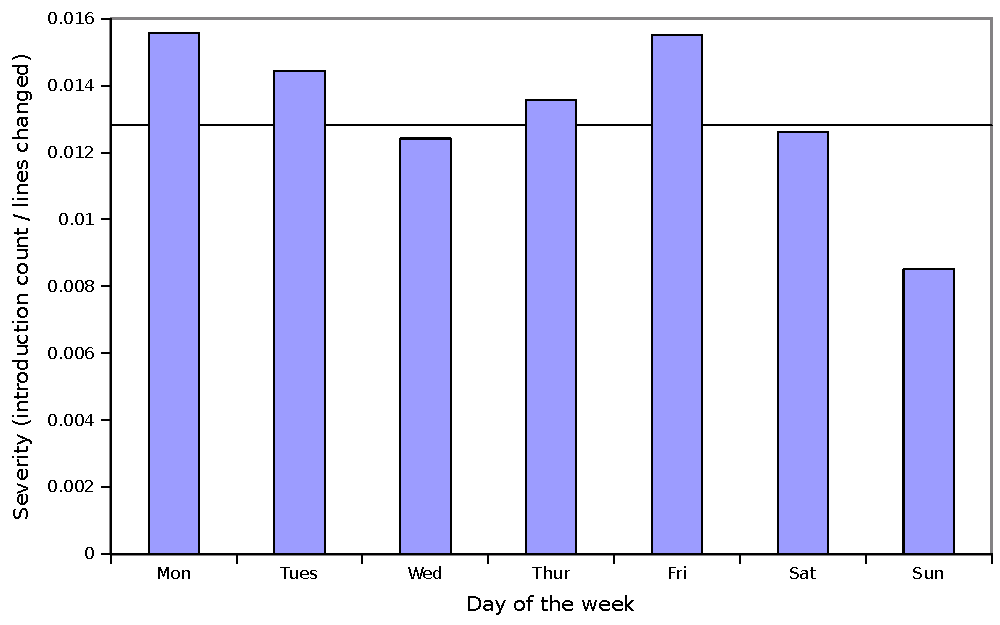
\includegraphics[width=\columnwidth]{postgresql-severity-day.pdf}
}
\caption{Severity of changes (bars) and average number of lines per commit (circles) versus day-of-week}
\label{fig-severity-day} % caption for the whole figure
\end{figure*}



%%  we
%% determine if the day of the week has any impact on the likelihood of
%% producing bugs. For the following graphs, the percentage of
%% introduction commits indicates the amount of commits which are bug
%% introductions, as a propostion of the total number of
%% commits. Figure~\ref{fig-linux-bugginess-day} presents our results for
%% the Linux kernel. We see that Saturday is the worst day, followed by Thursday,
%% while Monday has the fewest percentage of bug introductions. The
%% results for PostgreSQL are shown in Figure~\ref{fig-postgresql-bugginess-day} and
%% agree with Thursday being one of the worst days, while Monday is the
%% best day for committing changes which do not introduce bugs. 

%% A possible explanation is that developers rest over the weekend and have
%% ample time to think about the problem before coding a solution on
%% Monday, when they know exactly what to do. 

\subsection{Bug Lifetimes}
\label{sec-bug-lifetime}
Figures~\ref{fig-linux-bug-lifetime} and
\ref{fig-postgresql-bug-lifetime} show the bug lifetimes for the Linux
kernel and Postgres, with bug lifetimes grouped in 120 day
intervals. We found the average bug lifetime for the Linux kernel is
1.38 years with a standard deviation of 1.35 years. The average bug
lifetime for Postgres is 3.07 years with a standard deviation of 3.19
years. Postgres may have a longer average bug lifetime due to being a
smaller, less complex project with a smaller user base. We found the
sources of the long-time bugs include race conditions, incorrect
calculations and rare corner cases; such cases are intuitively more
likely to be found with a larger user base.  Note that the
distribution of bug lifetimes is similar for both projects; many bugs
are fixed within a 120 day period and the overall lifetime decreases
exponentially.

%---- lifetime 
\begin{figure*}[tbh]
\centering
\subfigure [ {Linux kernel} ]  
{
    \label{fig-linux-bug-lifetime}
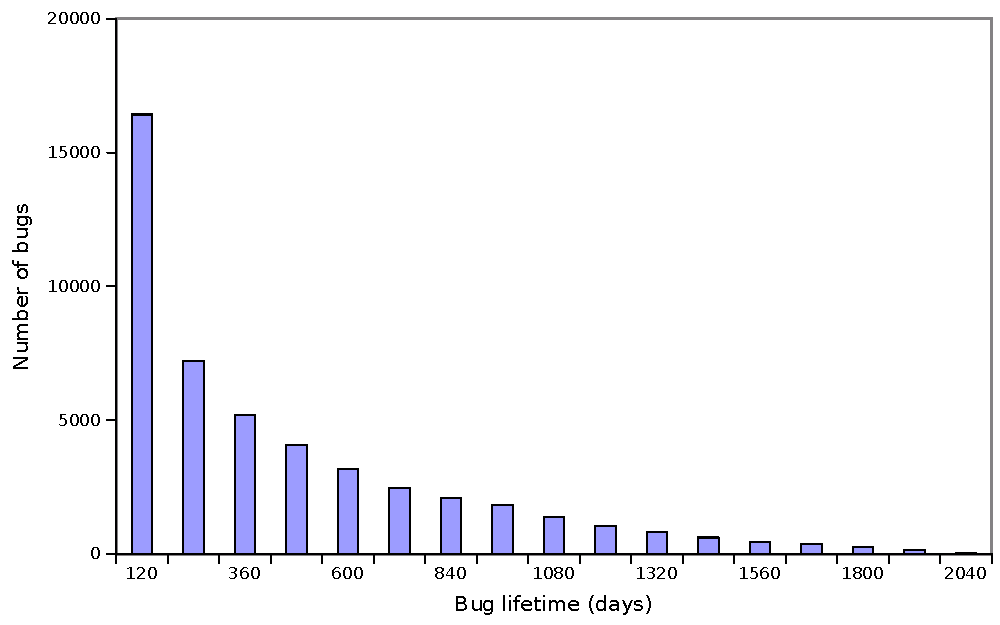
\includegraphics[width=\columnwidth]{linux-bug-lifetime.pdf}
}
\subfigure[ PostgreSQL ] 
{
    \label{fig-postgresql-bug-lifetime}
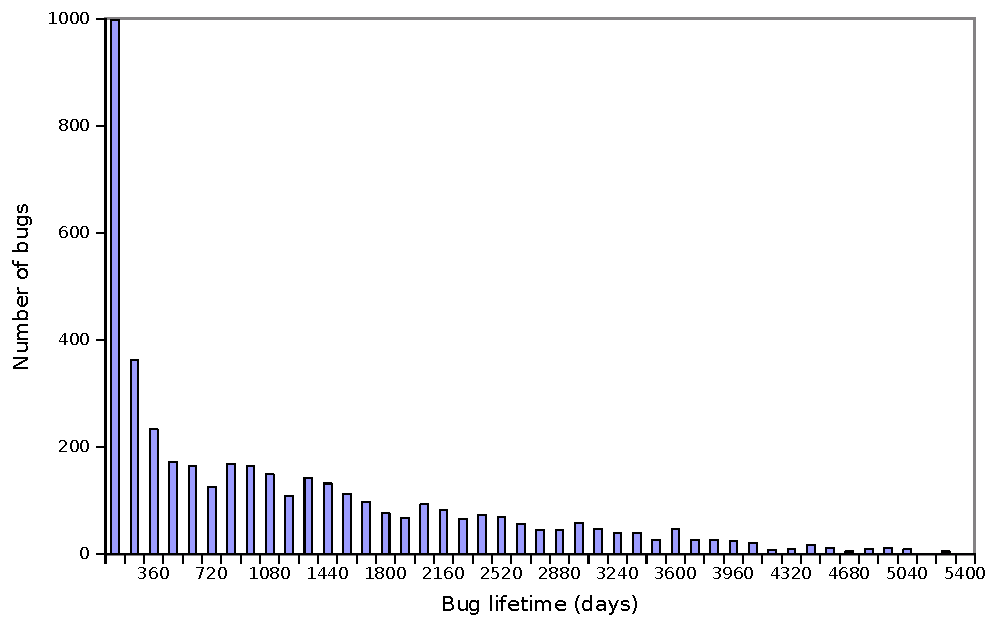
\includegraphics[width=\columnwidth]{postgresql-bug-lifetime.pdf}
}
\caption{Histogram of bug lifetime counts}
\label{fig-bug-lifetime} % caption for the whole figure
\end{figure*}

\subsection{Comment-only Commits}
\label{sec-comment-only}
A large number of bug-fixing commits in the database
reported 0 changed lines of code. We performed a random sample on 50 of these
commits for each project and found that almost all of them only changed comments in the
source code, which we did not count as changed lines of code. For the Linux kernel 
2.15~$\pm$~0.10\%~\footnote{We report
the margin of error with 95\% confidence level.} 
of the bug-fixing
commits (1,223 commits\footnote{Estimated based on the percentage of comment-only
commits and the total number of commits.}) were on comments only. We followed the same procedure for
PostgreSQL and found 2.97~$\pm$~0.45\% (estimated to be 131 commits) of bug-fixing commits were on
comments only.
These hundreds and thousands of comment-only commits show that developers spent time maintaining
the correctness of comments.

%% We also noted that approximately 7.7\% of the bug fixes for Linux were
%% purely for comments, indicating that developers spend a non-trivial
%% amount of time on comments. For Linux, approximately 51\% of the
%% changes do not include additions. We therefore manually checked (a
%% subsample of) the 49\% more difficult cases to evaluate the
%% effectiveness of our heuristic for additions.

\subsection{Validation} 
\label{sec-validation}
To validate our results, we estimated the precision and recall of our
technique for identifying bug-fixing commits on both projects.  As our
algorithm for identifying the associated bug-introducing commits was a
straightforward application of git blame, we did not systematically
verify its performance. (A brief manual inspection of bug-introducing
commits did not reveal any anomalies.) 
For both projects, we randomly sampled 50 bugs
from each of the population of commits that we identified to be
bug-introducing commits, BI (to evaluate precision).
%, and commits that we
%identified to be non-bug-fixing commits, $\neg$ BI (to evaluate recall).
Table~\ref{tab:pr-raw} summarizes our precision findings.
%and
%recall findings.

We evaluated the precision---that is, the proportion of identified
bug-fixing commits which do indeed fix bugs---and found that, for
the Linux kernel, 43 of the 50 bugs (in BI) that we automatically identified as
bug-fixing commits did indeed fix bugs, while 7 did not; for Postgres,
42 of 50 identified fixes (BI) were indeed fixes.  Some of the
cases included: 1) a commit message which fixed a merge commit was
classified as a fix; 2) apparently garbled commit messages which
included the keyword ``fix'' for no good reason; 3) changes which were
reverted (in the alleged ``fix'') but then re-added in a later
version; 4) poor uses of version control systems which included many
different changes in a single commit, including a fix as a small part 
of the commit; and 5) refactoring changes, which moved or renamed
functions---these could arguably be considered to be fixes to a buggy
initial design.

We have estimated our recall---the proportion of bug-fixing commits in
the entire sample that our technique identifies---to be at least \linuxR for
Linux and \postR for Postgres, and we are certain that our sampling
technique underestimates the recall. We intend to re-evaluate the
recall of our technique in the near future.

%% To evaluate the recall of our technique---the proportion of bug-fixing
%% commits in the entire sample that we manage to identify---we sampled
%% 50 non-bug-introducing commits from both the Linux kernel and
%% Postgres. Table~\ref{tab:pr-raw} presents the raw recall data. To compute
%% the recall, we evaluate
%% \[ \mbox{Recall} = \frac{\mbox{identified BI} \cap \mbox{actual BI}}{\mbox{identified BI}}; \]
%% however, to do so, we must normalize the number of identified bug-introducing
%% commits. Based on the precision results, we know that there are at least
%% 48745 bug-introducing commits, so we should have sampled 
%% Table~\ref{tab:pr-raw} therefore also shows our adjusted data in 
%% brackets.

\begin{table}
\begin{center}
\begin{tabular}{r|r|r}
& actual BI & actual $\neg$ BI \\ \hline
identified BI for Linux & 43 & 7 \\
%identified $\neg$ BI & 6 (23) & 44 (172) \\
%\end{tabular} 

%\begin{tabular}{r|r|r} Postgres & actual BI & actual $\neg$ BI \\ \hline
identified BI for Postgres & 42 & 8 \\
%identified $\neg$ BI & 3 (21) & 47 (332)
\end{tabular}
\end{center}
\caption{\label{tab:pr-raw}Results for precision. BI is bug-introducing commits.}

%% \begin{center}
%% \begin{tabular}{rrr}
%% Linux & actual BI & actual $\neg$ BI \\
%% identified BI & 43 & 7 \\
%% identified $\neg$ BI & 23 & 172 \\
%% \end{tabular} 

%% \begin{tabular}{rrr} Postgres & actual BI & actual $\neg$ BI \\
%% identified BI & 42 & 8 \\
%% identified $\neg$ BI & 21 & 332
%% \end{tabular}
%% \end{center}
%% \caption{\label{tab:pr-adj}Adjusted results for precision and recall.}
\end{table}


